\item A particle of mass \( m \) moves along a circle of radius \( R \). Find the modulus of the average vector of the force acting on the particle over the distance equal to a quarter of the circle, if the particle moves
    \begin{enumerate}
        \item uniformly with velocity \( v \);
        \item with constant tangential acceleration \( w_{\tau} \), the initial velocity being equal to zero.
    \end{enumerate}
    \begin{center}
        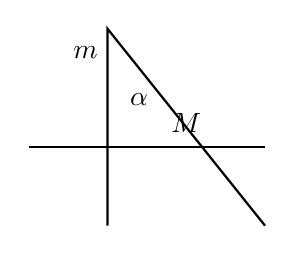
\begin{tikzpicture}
            \draw [thick] (-1,0) -- (2,0);
            \draw [thick] (0,-1) -- (0,1.5) -- (2,-1);
            \node at (1,0.3) {\( M \)};
            \node at (0,1) [above left] {\( m \)};
            \node at (0.4,0.6) {\( \alpha \)};
        \end{tikzpicture}
    \end{center}\begin{solution}
    \begin{center}
        \begin{tikzpicture}
            \pic at (0, 0) {frame=3cm};
        \end{tikzpicture}
    \end{center}
    
    \begin{align*}
        \intertext{Let us sketch the diagram for the motion of the particle of mass $m$ along the circle of radius $R$ as shown in the figure.}
        \intertext{For a particle, modulus of change in linear momentum $\lvert \Delta\vec{p} \rvert = m \lvert \Delta\vec{v} \rvert$.}
        \intertext{(a) In this case $|\Delta \vec{v}| = \sqrt{2}v$ (see figure), and the time taken in describing quarter of the circle,}
        \Delta t &= \frac{\pi R}{2v}\\
        \intertext{Hence,}
        \left\lvert <\vec{F}> \right\rvert &= \frac{|\Delta \vec{p}|}{\Delta t} = \frac{m|\Delta \vec{v}|}{\Delta t}\\
        &= \frac{\sqrt{2}mv}{\pi R / 2v} = \frac{2 \sqrt{2} mv^2}{\pi R}\\
        \intertext{(b) In this case $\vec{v}_i = 0$, so $\vec{v}_f = \vec{v}(t)$. Thus $|\Delta \vec{v}| = |\vec{v}(t)| = v(t) = w_t t$.}
        \intertext{Hence,}
        \left\lvert <\vec{F}> \right\rvert &= \frac{|\Delta \vec{p}|}{\Delta t} = \frac{m|\Delta \vec{v}(t)|}{t} = mw_t
    \end{align*}
\end{solution}